\subsection{MEX 2-4: Large wellbore test (Springen)}

Participating institutions of MEX 2-4 (see section \ref{sec:mex11}): IfG

\begin{table}[ht!]
\caption{MEX 2-4: Data overview}
\label{tab:dms-mex24-overview}
\small
\begin{tabular}{l|l|l|l|L{4.7cm}|l}
\hline
\rowcolor{cyan}
Type & Spec. & Owner & Access     & Comment                       & Stat \\ 
\hline 
EXP  & URL   & IfG   & Restricted & Available on demand           & \cellcolor{green} \\
\hline \hline
MOD  & DEM   & IfG   & License    & Commercial software           & \cellcolor{green} \\
     &       &       & Restricted & I/O available on demand       & \cellcolor{green} \\
\hline
\end{tabular}
\end{table}
\normalsize

%---------------------------------------------------------
\subsubsection*{Meta Data Overview (according to Dublin Core)}
%---------------------------------------------------------

\begin{table}[!ht]
\caption{MEX 2-4 (IfG)}
\label{tab:dms-mex2-4}
\small
\begin{tabular}{R{3.5cm}|L{7cm}}
\hline
%
Data label              & GeomInt, MEX 2-4, IfG, large wellbore test, URL Springen \\
URL                     & In-house data storage \\
Subject                 & Integrity, tidiness of salt rocks for different fluids (gases and brines) \\
Type of data            & Dataset (structured data in a defined format) \\
Data quality            & Quality assured data \\
Status of data          &  \\
Data format             & ASCII \\
Creators                & IfG GmbH \\
Source/Origin           & IfG GmbH \\
Publisher               & IfG GmbH, Friederikenstra\ss e 60, 04279 Leipzig\\
Rights holders          & IfG GmbH, Friederikenstra\ss e 60, 04279 Leipzig \\
Contributors            & Mathias Nest \\
Time/period of creation & 2018-2019 \\
Language of the content & German \\
Update policy           & Ongoing updates \\
Access permissions      & Limited access \\
%
\hline
\end{tabular}
\end{table}

\begin{wrapfigure}{l}{5cm}
\centering
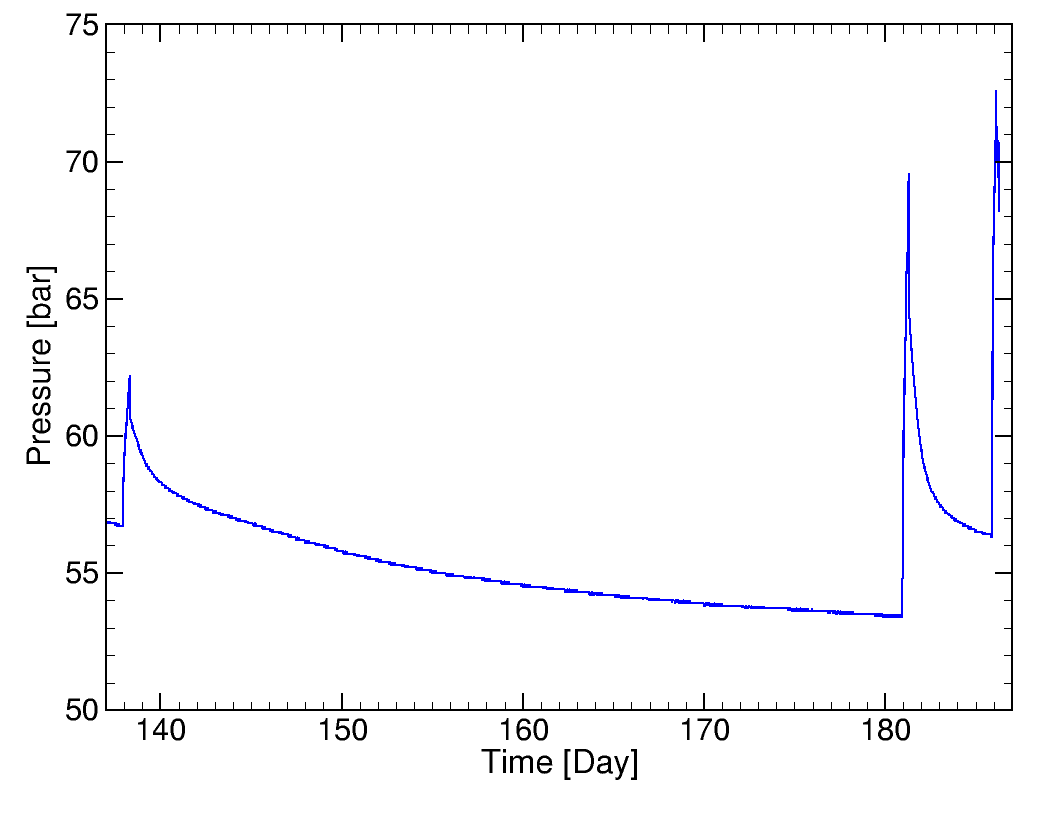
\includegraphics[width=5cm]{figures/IfG-Druckkurve-50d.png}
\caption{Measured pressure curve data: $p(t)$}
\label{fig:dms-mex24}
\end{wrapfigure}

The data set contains a measured pressure curve over time (50 days) during an injection test in a large wellbore (Springen URL). The injection regime was conducted in 5 bar increasing pressure steps followed by shut-in periods for observing the related pressure diffusion. Corresponding pumping rates were between 1-5.5 liters per second. Peak pressures of more than 60 bars were required to create in-situ discontinuities by overcoming the tensile/adhesive rock strength of salt. Additionally, acoustic emission (AE) data were recorded.